\newprob{1715746133}
{
    湯姆使用電水壼煮1.2升的水。電水壼的輸出功率是2.2 kW。
    \begin{parts}
        \part[2] 把1.2升的水從 \oc{25} 煮到沸騰需要多少時間?
        \par 已知:1升水的質量 = 1 kg
        ,水的比熱容量 = \shc{4200}
        % \fillwithdottedlines{2.5in}
        \part[2] 開啓電水壼的的電源,水在3分20秒之後開始沸騰。
        \begin{subparts}
            \subpart 假設每kWh的電費為\$1.2,計算煮這壺水所需的電費。($\qty{1}{kWh}=1000\times$\qty{3600}{J})
            \subpart 茶壺所提供的能量中,有多少百分比會轉化為水的內能?
            % \fillwithdottedlines{\stretch{1}}
        \end{subparts}
    \end{parts}
}{

}

\newprob{1715746528}
{
    傑森的家裡有一個漂亮的水族箱。由於室溫的變化,水溫在一個晚上從 \oc{25}下降到 \oc{21}。
    \begin{parts}
        \part[2] 水族箱系統內有 \qty{100}{kg}的水。問有多少能量從水中被帶走了?
        % \fillwithdottedlines{2.in}
        \part[2] 傑森將一個功率為 \qty{100}{W}的水族箱加熱器放入水槽中。需要多長時間才能將水加熱回 \oc{25}?假設沒有熱散失在周圍環境。
        % \fillwithdottedlines{2.5in}
        \part[2] 你預計在問題(b)中得到的加熱時間會比實際加熱時間更長、相等還是更短?請簡要解釋你的答案。
        % \fillwithdottedlines{\stretch{1}}
    \end{parts}
}{}

\newprob{1715747654}
{
    一個學生設計了一個實驗,通過混合法來確定一種新材料的比熱容。已知質量的水被放置在一個良好隔熱的鋁罐中。實驗設置如圖中所示。記錄水的初始溫度。然後樣品在烤箱中加熱到$200^{\circ}$C,然後迅速轉移到鋁罐中。攪拌均勻後,測量水的最終穩定溫度。
    % \par A student has designed an experiment to determine the specific heat capacity of a new material using the method of mixing. A known mass of water is placed in a well-insulated aluminum can. The experimental setup is shown in the diagram. The initial temperature of the water is recorded. Then, the sample is heated to $200^{\circ}C$ in an oven and quickly transferred to the aluminum can. After thorough mixing, the final stable temperature of the water is measured.
    \begin{figure}[h]
        \centering
        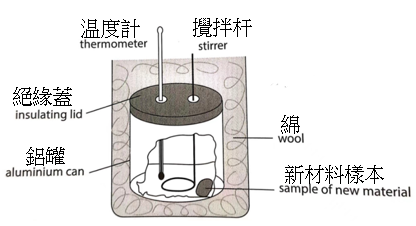
\includegraphics[width=0.5\linewidth]{assets/Screenshot_9.png}
    \end{figure}
    \par 樣品質量 = $16.0$g
    \par 空鋁罐的質量 = $60.0$g
    \par 帶水的罐子的質量 = $160.0$g
    \par 水的初始溫度 = $25.0^\circ$C
    \par 水的最終溫度 = $27.3^{\circ}$C
    \par \medskip  已知:鋁的比熱容= \shc{987}, 水的比熱容= \shc{4200}
    % \par Given: specific heat capacity of Aluminium = \shc{987}, that of water=\shc{4200}
    \begin{parts}
        \part[2] 計算該材料的比熱容。
        % \par Calculate the specific heat capacity of the material.
        % \fillwithlines{\stretch{1}}
        % \clearpage
        \part[2] 最初,這個學生建議將樣品放在沸水中加熱到\oc{100},然後再將其轉移到水中的罐中。列出她建議的兩個缺點。
        % \par Originally, Anne suggested to heat the sample to \oc{100} by placing it in boiling water before it is transferred to the can of water. State two disadvantages of following her suggestion.
        % \fillwithlines{2.5in}
        \medskip
        \part[2] 列出她采取的兩項預防措施以減少熱量散失到周圍環境。
        % \par State two precautions that she has taken to reduce heat lost to the surroundings.
        % \fillwithlines{2.5in}
    \end{parts}
}{}

\newprob{1715747738}
{
    一名學生進行了一個簡單的實驗,估計本生燈火焰的最熱部分。他用有絕緣手柄的鉗子拿著一小塊鎢,將其放在火焰的中央部分加熱幾分鐘。然後,他迅速地將鎢塊放入一個裝有一些水的發泡膠杯中。記錄了混合物的最終最高溫度。得到以下結果。
    % \par A student performed a simple experiment to estimate the hottest part of a Bunsen flame. A small lump of tungsten was held by tongs (with insulating handles) and heated in the middle of the flame for a few minutes. Then the lump was quickly dropped into a polystyrene cup containing some water. The final maximum temperature of the mixture was recorded. The following results were obtained.
    \par 鎢的質量 = \qty{12.0}{g},
    發泡膠杯中的水的質量 = \qty{135}{g},
    水的初始溫度 = \oc{20.0},
    混合後水的最終溫度 = \oc{23.1},
    已知數據:鎢的比熱容 = \shc{134}; 水的比熱容 = \shc{4200}

    \begin{parts}
        \part[2] 忽略發泡膠杯的熱容,估計本生火焰的溫度。
        % \par Neglecting the heat capacity of the polystyrene cup, estimate the temperature of the Bunsen flame from these data.
        % \fillwithlines{3in}

        \part[2] 從(a)中得到的答案是高於還是低於火焰的最高溫度?試提出兩個原因解釋。
        % \par Is answer in (a) higher or lower than the maximum temperature of the flame? Why? Suggest two reasons to explain your answer.
        % \fillwithlines{3in}
        \part[1] 試提出一種更準確的方法來確定本生火焰的最高溫度。
        % \par Suggest a more accurate method to determine the maximum temperature of the Bunsen flame.
        % \fillwithlines{1in}

    \end{parts}
}{}

\newprob{1715747826}
{

}{}